% ============================================================
\chapter{THẢO LUẬN}
\label{ch:thao_luan}
% ============================================================

\section{Vì sao trọng số lớp đơn thuần không hiệu quả?}

Kết quả Exp 2 ($-0{,}45$ pp so với baseline) thoạt nhìn nghịch lý, nhưng phù hợp với
lý thuyết. Trọng số nghịch tần suất nâng gradient của lớp hiếm lên rất cao
(Bảng~\ref{tab:imbalance}: Fence $= 7{,}22$, Car $= 2{,}03$), khiến mô hình "cố gắng"
dự đoán các lớp này ở cả những vùng không chắc chắn $\Rightarrow$ tăng dương tính giả
và \textbf{xâm lấn} sang lớp phổ biến. Quan sát trong Bảng~\ref{tab:perclass} xác
nhận: Fence/Car tăng nhưng Building, Deciduous, Coniferous, Rocks đều giảm. Tổng hợp
lại, phần mất ở lớp phổ biến lớn hơn phần được ở lớp hiếm, kéo mIoU xuống.

\section{Vì sao tổ hợp Focal+Dice+CE hiệu quả hơn?}

Hai cơ chế bổ trợ giải thích ưu thế của Exp 3 và Exp 4:
\begin{itemize}[leftmargin=1.4cm]
  \item \textbf{Focal Loss} tập trung vào điểm ảnh khó (biên, vật thể nhỏ) thay vì
  ép theo tần suất lớp, nên ít gây dương tính giả hơn trọng số cứng.
  \item \textbf{Dice Loss} tối ưu trực tiếp độ chồng lấp vùng và bất biến với kích
  thước lớp, giúp lớp nhỏ (Fence, Car) đóng góp tương xứng vào mục tiêu tối ưu mà
  không bóp méo lớp lớn.
\end{itemize}
Sự kết hợp này nâng lớp hiếm \emph{và} bảo toàn lớp phổ biến --- điều mà trọng số CE
đơn thuần không làm được.

\section{Giá trị của cơ chế thích nghi}

Exp 4 vượt trội nhờ \emph{học} tỷ trọng giữa ba thành phần loss thay vì cố định. Cơ
chế bất định đa nhiệm~\cite{kendall2018uncertainty} cho phép mô hình tự giảm ảnh
hưởng của thành phần "nhiễu" theo từng giai đoạn huấn luyện. Kết quả là Exp 4 đạt IoU
cao nhất trên \emph{toàn bộ} lớp hiếm đồng thời khôi phục gần như hoàn toàn hiệu năng
lớp phổ biến (xem Bảng~\ref{tab:perclass}).

\section{Phân tích lỗi vật thể nhỏ}

Phân tích chi tiết (recall, precision, nhầm lẫn) cho các lớp nhỏ cho thấy lỗi phổ
biến là \emph{nhầm sang Ground\_vegetation} --- lớp nền chiếm ưu thế. Ví dụ với
baseline, một phần đáng kể điểm ảnh Fence và Fallen\_trees bị gán nhầm thành
Ground\_vegetation. Các chiến lược Focal+Dice giảm đáng kể kiểu lỗi này.

\begin{figure}[H]
\centering
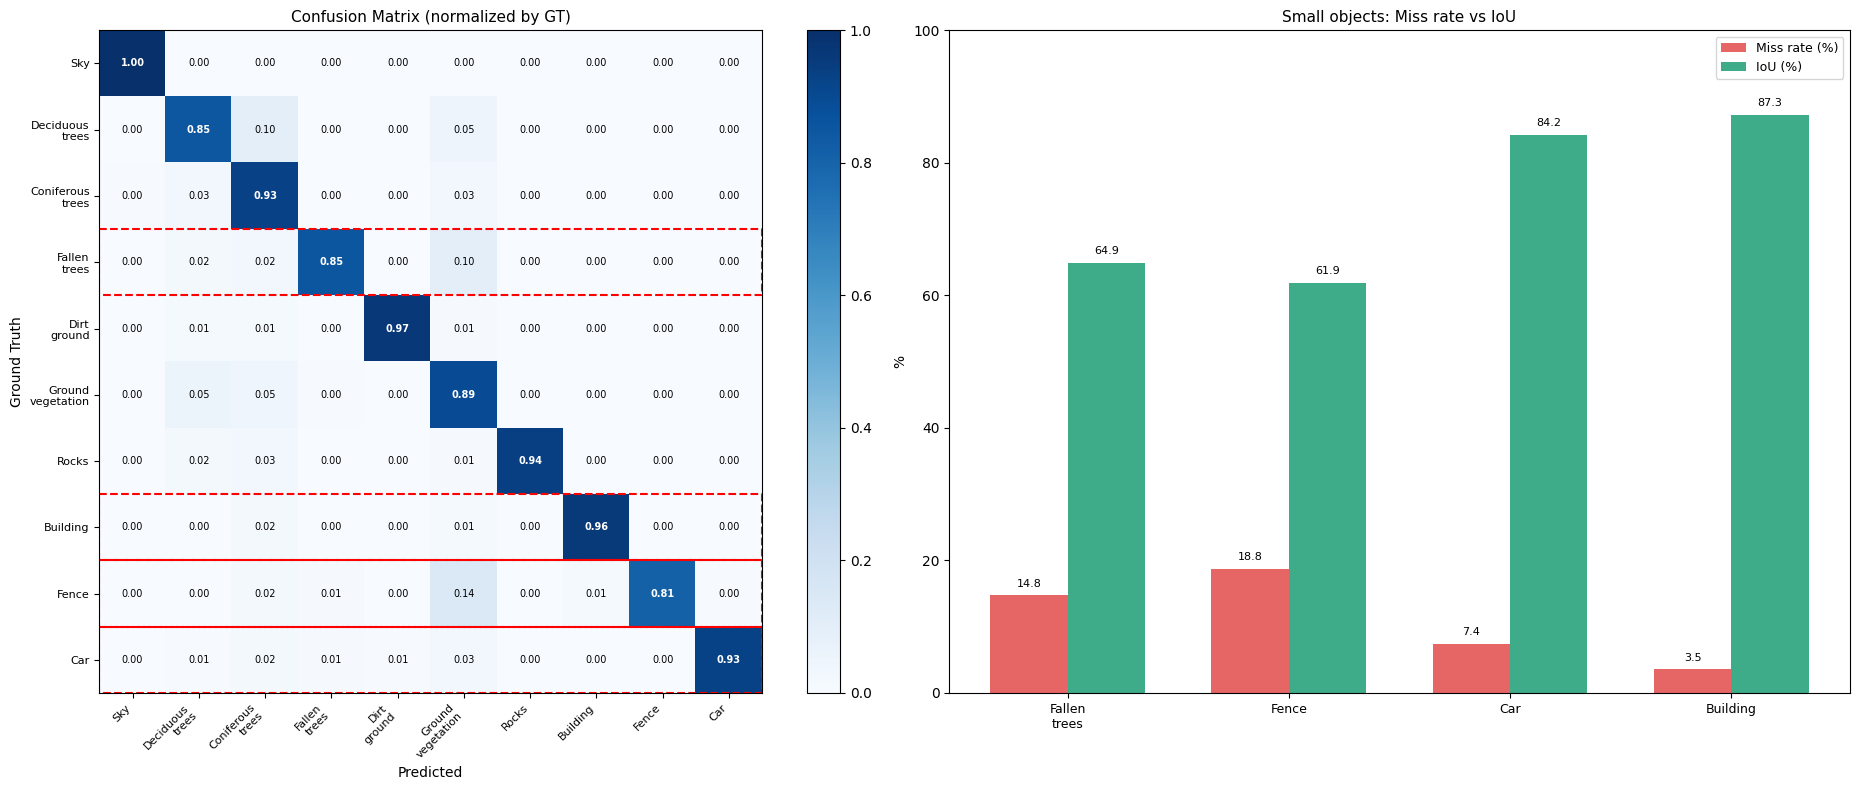
\includegraphics[width=\textwidth]{figures/fig_confusion_smallobj.png}
\caption{Trái: ma trận nhầm lẫn chuẩn hóa theo nhãn chuẩn (10 lớp). Phải: tỷ lệ bỏ
sót (miss rate) và IoU của bốn lớp nhỏ/hiếm. Lỗi phổ biến nhất là nhầm Fence và Fallen
trees sang Ground vegetation (cột tương ứng trong ma trận).}
\label{fig:confusion}
\end{figure}

\section{Hạn chế và mối đe dọa tới tính hợp lệ}
\label{sec:han_che}

Để bảo đảm tính nghiêm túc khoa học, báo cáo nêu rõ các hạn chế sau:

\begin{enumerate}[leftmargin=1.4cm]
  \item \textbf{Số epoch chưa đồng nhất.} Exp 4 huấn luyện 100 epoch trong khi Exp
  1--3 chỉ 50 epoch; một phần ưu thế của Exp 4 có thể đến từ thời gian huấn luyện dài
  hơn. \emph{Khắc phục:} chạy lại Exp 4 ở 50 epoch (hoặc Exp 1--3 ở 100 epoch) để so
  sánh tách bạch ảnh hưởng của loss.
  \item \textbf{Giao thức đánh giá chưa thống nhất.} Exp 1 và Exp 4 đánh giá bằng
  \emph{checkpoint tốt nhất}, còn Exp 2 và Exp 3 đánh giá bằng \emph{mô hình ở epoch
  cuối}. \emph{Khắc phục:} thống nhất dùng checkpoint tốt nhất cho cả bốn.
  \item \textbf{Mới một seed cho Exp 4.} Kết quả $0{,}8365$ là của seed 2025; cần
  bổ sung seed 42 và 123 để báo cáo trung bình $\pm$ độ lệch chuẩn
  (Mục~\ref{sec:multiseed}).
  \item \textbf{Cách chia dữ liệu đặc thù.} Tập kiểm thử \{seq6, seq7\} chứa chuỗi
  chụp ngang (nhiều Sky), khiến mIoU cao và không so trực tiếp được với benchmark
  dùng cách chia khác (Mục~\ref{sec:split}).
  \item \textbf{Dữ liệu mô phỏng.} Bộ dữ liệu sinh từ AirSim; khả năng tổng quát hóa
  sang ảnh thực cần kiểm chứng qua WildUAV (Mục~\ref{sec:wilduav}).
  \item \textbf{Một kiến trúc.} Kết luận giới hạn ở UNet++/ResNet50; cần xác nhận
  trên các kiến trúc khác (Mục~\ref{sec:multi_arch}).
\end{enumerate}
